\begin{table*}[th]
    \centering
    \tiny
    \resizebox{\linewidth}{!}{
        \begin{tabular}{cccccccc}
        \hline
        \textbf{Case} & \textbf{Character} & \textbf{Initial} & \textbf{Final} & \textbf{Rule} & \textbf{Initial IPA} \\
        \hline
        direct                      & \begin{CJK*}{UTF8}{gbsn}波\end{CJK*} &  \begin{CJK*}{UTF8}{gbsn}帮\end{CJK*} & \begin{CJK*}{UTF8}{gbsn}戈\end{CJK*} & \begin{CJK*}{UTF8}{gbsn}帮\end{CJK*}=[p] and \begin{CJK*}{UTF8}{gbsn}戈\end{CJK*}=[\textipa{uA}] & [p] \\
        \multirow{2}{*}{rule-based} 
        & \begin{CJK*}{UTF8}{gbsn}砩\end{CJK*} & \begin{CJK*}{UTF8}{gbsn}帮\end{CJK*} & \begin{CJK*}{UTF8}{gbsn}废\end{CJK*} & \multirow{2}{*}{if(initial=\begin{CJK*}{UTF8}{gbsn}帮\end{CJK*} and final=\begin{CJK*}{UTF8}{gbsn}废\end{CJK*}) then [f] else [p]} & [f] \\
        & \begin{CJK*}{UTF8}{gbsn}碑\end{CJK*} & \begin{CJK*}{UTF8}{gbsn}帮\end{CJK*} & \begin{CJK*}{UTF8}{gbsn}支\end{CJK*} &  & [p] \\
        arbitrary                   & \begin{CJK*}{UTF8}{gbsn}方\end{CJK*} & \begin{CJK*}{UTF8}{gbsn}帮\end{CJK*} & \begin{CJK*}{UTF8}{gbsn}阳\end{CJK*} & - & [f] \\
        \hline
        converted                   & \begin{CJK*}{UTF8}{gbsn}比\end{CJK*} & \begin{CJK*}{UTF8}{gbsn}帮\end{CJK*} & \begin{CJK*}{UTF8}{gbsn}旨\end{CJK*} & - & [p]\\
        \hline				
        \end{tabular}
        }
    \caption{Five different examples of reconstruction.}
    \label{tab:reconstruction}
\end{table*}
\section{Different Cases of Reconstruction}
\label{app:reconstruction}
\tabref{tab:reconstruction} presents five examples in four different cases constructing our ancient Chinese pronunciation dataset for each category. For an identical initial category, different rules applied can lead to different reconstruction result for initial IPA.

\section{Embedding for Medial Feature, Nucleus Feature, and Coda Feature}
\label{app:embedding}
This appendix supplements the embedding employed for the medial, nucleus, and coda features in GTenhanced Transformer, as shown in \figref{fig:embedding2}.

\begin{figure*}[th]
    \centering
    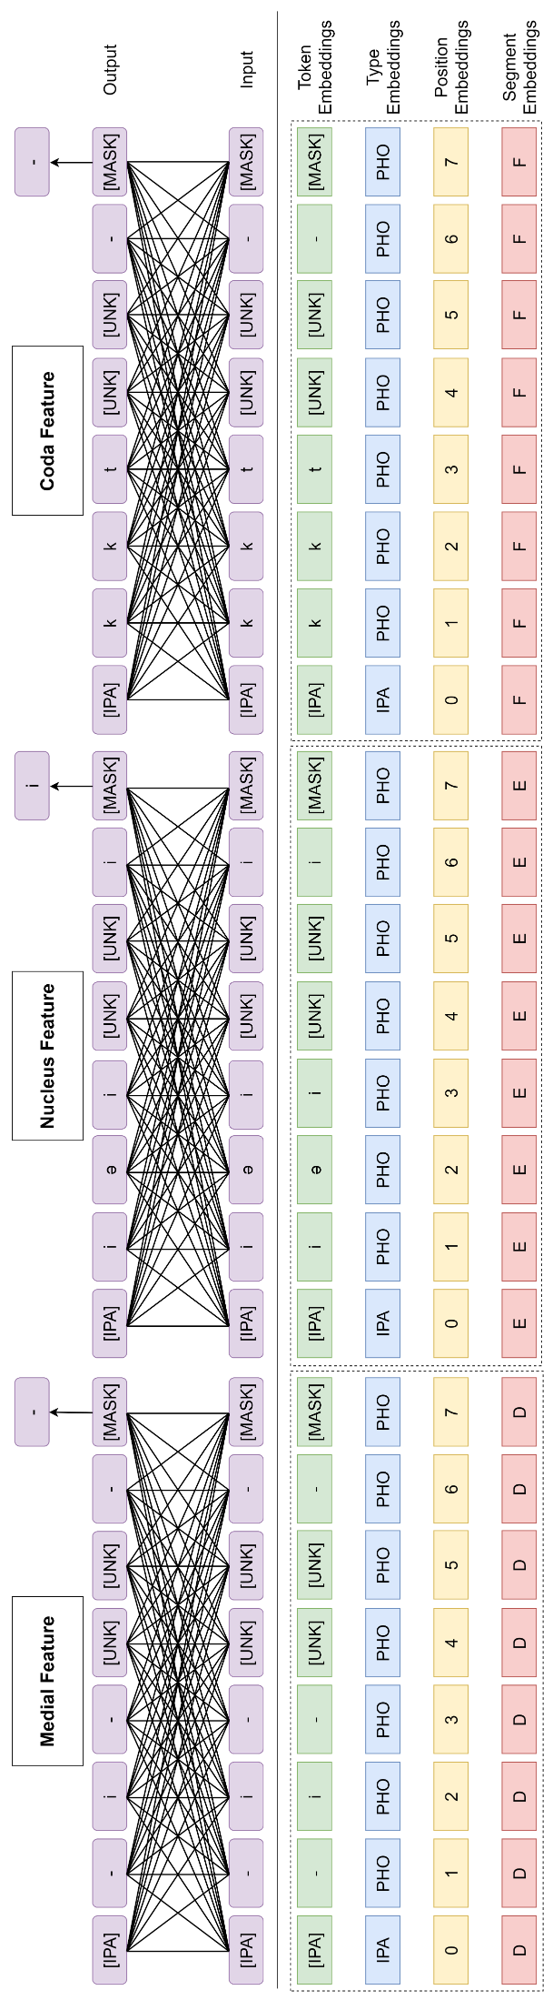
\includegraphics[width=0.4\textwidth]{images/embedding_layer2.png}
    \caption{Embedding for medial feature, nucleus feature, and coda feature.}
    \label{fig:embedding2}
\end{figure*}

